% !TEX TS-program = pdflatex
% !TEX encoding = UTF-8 Unicode

%%%%%%%%%%%%%%%%%%%%%%%%%%%%%%%%%%%%%%%%%
% Structured General Purpose Assignment
% LaTeX Template
%
% This template has been downloaded from:
% http://www.latextemplates.com
%
% Original author:
% Ted Pavlic (http://www.tedpavlic.com)
%
% Note:
% The \lipsum[#] commands throughout this template generate dummy text
% to fill the template out. These commands should all be removed when 
% writing assignment content.
%
%%%%%%%%%%%%%%%%%%%%%%%%%%%%%%%%%%%%%%%%%

%----------------------------------------------------------------------------------------
%	PACKAGES AND OTHER DOCUMENT CONFIGURATIONS
%----------------------------------------------------------------------------------------

\documentclass[12pt]{article}
\usepackage[utf8]{inputenc} % set input encoding (not needed with XeLaTeX)

\usepackage{fancyhdr} % Required for custom headers
\usepackage{lastpage} % Required to determine the last page for the footer
\usepackage{extramarks} % Required for headers and footers
\usepackage{graphicx} % Required to insert images
\usepackage{caption}
\usepackage{float}
\usepackage{listings}
\usepackage{url}
\usepackage{subcaption}
\usepackage{amssymb}
\usepackage{textcomp}
\usepackage{color}
\usepackage{pdfpages}
\usepackage[hidelinks]{hyperref}
\usepackage{tikz}

\def\checkmark{\tikz\fill[scale=0.4](0,.35) -- (.25,0) -- (1,.7) -- (.25,.15) -- cycle;} 

\definecolor{lightgray}{rgb}{.9,.9,.9}
\definecolor{darkgray}{rgb}{.4,.4,.4}
\definecolor{purple}{rgb}{0.65, 0.12, 0.82}

\lstdefinelanguage{JavaScript}{
  keywords={typeof, new, true, false, catch, function, return, null, catch, switch, var, if, in, while, do, else, case, break},
  keywordstyle=\color{blue}\bfseries,
  ndkeywords={class, export, boolean, throw, implements, import, this},
  ndkeywordstyle=\color{darkgray}\bfseries,
  identifierstyle=\color{black},
  sensitive=false,
  comment=[l]{//},
  morecomment=[s]{/*}{*/},
  commentstyle=\color{purple}\ttfamily,
  stringstyle=\color{red}\ttfamily,
  morestring=[b]',
  morestring=[b]"
}

\lstset{
   language=JavaScript,
   backgroundcolor=\color{lightgray},
   extendedchars=true,
   basicstyle=\footnotesize\ttfamily,
   showstringspaces=false,
   showspaces=false,
   numbers=left,
   numberstyle=\footnotesize,
   numbersep=9pt,
   tabsize=2,
   breaklines=true,
   showtabs=false,
   captionpos=b
}

\hypersetup{colorlinks=false}

% Margins
\topmargin=-0.45in
\evensidemargin=0in
\oddsidemargin=0in
\textwidth=6.5in
\textheight=9.0in
\headsep=0.25in 


\linespread{1.1} % Line spacing

% Set up the header and footer
\pagestyle{fancy}
\lhead{\hmwkAuthorName} % Top left header
\chead{\hmwkClass\ \hmwkTitle} % Top center header
\rhead{\firstxmark} % Top right header
\lfoot{\lastxmark} % Bottom left footer
\cfoot{} % Bottom center footer
\rfoot{Page\ \thepage\ of\ \pageref{LastPage}} % Bottom right footer
\renewcommand\headrulewidth{0.4pt} % Size of the header rule
\renewcommand\footrulewidth{0.4pt} % Size of the footer rule

\setlength\parindent{0pt} % Removes all indentation from paragraphs

%----------------------------------------------------------------------------------------
%	DOCUMENT STRUCTURE COMMANDS
%	Skip this unless you know what you're doing
%----------------------------------------------------------------------------------------

% Header and footer for when a page split occurs within a problem environment
\newcommand{\enterProblemHeader}[1]{
\nobreak\extramarks{#1}{#1 continued on next page\ldots}\nobreak
\nobreak\extramarks{#1 (continued)}{#1 continued on next page\ldots}\nobreak
}

% Header and footer for when a page split occurs between problem environments
\newcommand{\exitProblemHeader}[1]{
\nobreak\extramarks{#1 (continued)}{#1 continued on next page\ldots}\nobreak
\nobreak\extramarks{#1}{}\nobreak
}

\setcounter{secnumdepth}{0} % Removes default section numbers
\newcounter{homeworkProblemCounter} % Creates a counter to keep track of the number of problems

\newcommand{\homeworkProblemName}{}
\newenvironment{homeworkProblem}[1][Problem \arabic{homeworkProblemCounter}]{ % Makes a new environment called homeworkProblem which takes 1 argument (custom name) but the default is "Problem #"
\stepcounter{homeworkProblemCounter} % Increase counter for number of problems
\renewcommand{\homeworkProblemName}{#1} % Assign \homeworkProblemName the name of the problem
\section{\homeworkProblemName} % Make a section in the document with the custom problem count
\enterProblemHeader{\homeworkProblemName} % Header and footer within the environment
}{
\exitProblemHeader{\homeworkProblemName} % Header and footer after the environment
}

\newcommand{\problemAnswer}[1]{ % Defines the problem answer command with the content as the only argument
\noindent\framebox[\columnwidth][c]{\begin{minipage}{0.98\columnwidth}#1\end{minipage}} % Makes the box around the problem answer and puts the content inside
}

\newcommand{\homeworkSectionName}{}
\newenvironment{homeworkSection}[1]{ % New environment for sections within homework problems, takes 1 argument - the name of the section
\renewcommand{\homeworkSectionName}{#1} % Assign \homeworkSectionName to the name of the section from the environment argument
\subsection{\homeworkSectionName} % Make a subsection with the custom name of the subsection
\enterProblemHeader{\homeworkProblemName\ [\homeworkSectionName]} % Header and footer within the environment
}{
\enterProblemHeader{\homeworkProblemName} % Header and footer after the environment
}
   
%----------------------------------------------------------------------------------------
%	NAME AND CLASS SECTION
%----------------------------------------------------------------------------------------

\newcommand{\hmwkTitle}{`MyAlcoholFreeWine.com'} % Assignment title
\newcommand{\hmwkDueDate}{Monday,\ December\ 7,\ 2015} % Due date
\newcommand{\hmwkClass}{SE31520} % Course/class
\newcommand{\hmwkAuthorName}{James Euesden - jee22} % Your name

%----------------------------------------------------------------------------------------
%	TITLE PAGE
%----------------------------------------------------------------------------------------

\title{
\vspace{2in}
\textmd{\textbf{\hmwkClass:\ \hmwkTitle}}\\
\normalsize\vspace{0.1in}\small{Due\ on\ \hmwkDueDate}\\
\vspace{3in}
}

\author{\textbf{\hmwkAuthorName}}
\date{} % Insert date here if you want it to appear below your name

%----------------------------------------------------------------------------------------

\setlength\parindent{24pt}

\begin{document}

\maketitle

%----------------------------------------------------------------------------------------
%	TABLE OF CONTENTS
%----------------------------------------------------------------------------------------

%\setcounter{tocdepth}{1} % Uncomment this line if you don't want subsections listed in the ToC

\newpage
\tableofcontents
\newpage

%----------------------------------------------------------------------------------------
%	INTRODUCTION
%----------------------------------------------------------------------------------------

% To have just one problem per page, simply put a \clearpage after each problem

\section{Introduction}

The assignment task\cite{assignment} was to implement a web site using Ruby on Rails, and a Web Service with RESTful resources. The web site, MyAlcoholFreeWines.com (MAF), was to call two instances of the Web Service as Wine Suppliers, get their list of Wines and then display to a Customer the cheapest wines available, and place an order them if they wished. This report serves to document the design, testing and structure of my application, and as self evaluation of work carried out. All Wine images used for the application are credited to StockVault\cite{stockvault} from their Free Wine Stock Photos gallery.

%----------------------------------------------------------------------------------------
%	MAF ARCHITECTURE
%----------------------------------------------------------------------------------------

\section{MAF Architecture}
For the MAF, I knew that I had to have some way of storing the Wines when I got results back from the Web Services. I considered I could keep them in memory, which might be okay for a very small application, but is completely un-scalable for an application that could be used by many and with multiple massively stocked Wine Suppliers. I chose to keep the Wines received in a Database and represent them as entities, where I would store all Wines provided by each supplier, but only the cheapest of each Wine.

The preliminary design of the application was based on the example provided in the `Agile Web Development with Rails'\cite{railsbook} book, and then modified to meet the requirements. This was a good starting place for learning how to implement Sessions and Baskets as I was very new to Rails and lacked understanding to implement it at the start of this assignment.

My main entities in the design for MAF are Wines, Customer, CustomerDetail, Basket and BasketItem. These all have their own controllers, views and models. There is also a controller for Sessions, which refers to when a Customer is on the website and has a `session', allowing them to be logged in and retain a Basket with BasketItems as they navigate through the site, until their session ends.

You can see below what my design for the database entities and their relationships were when I started.

\begin{figure}[H]
        \centering
                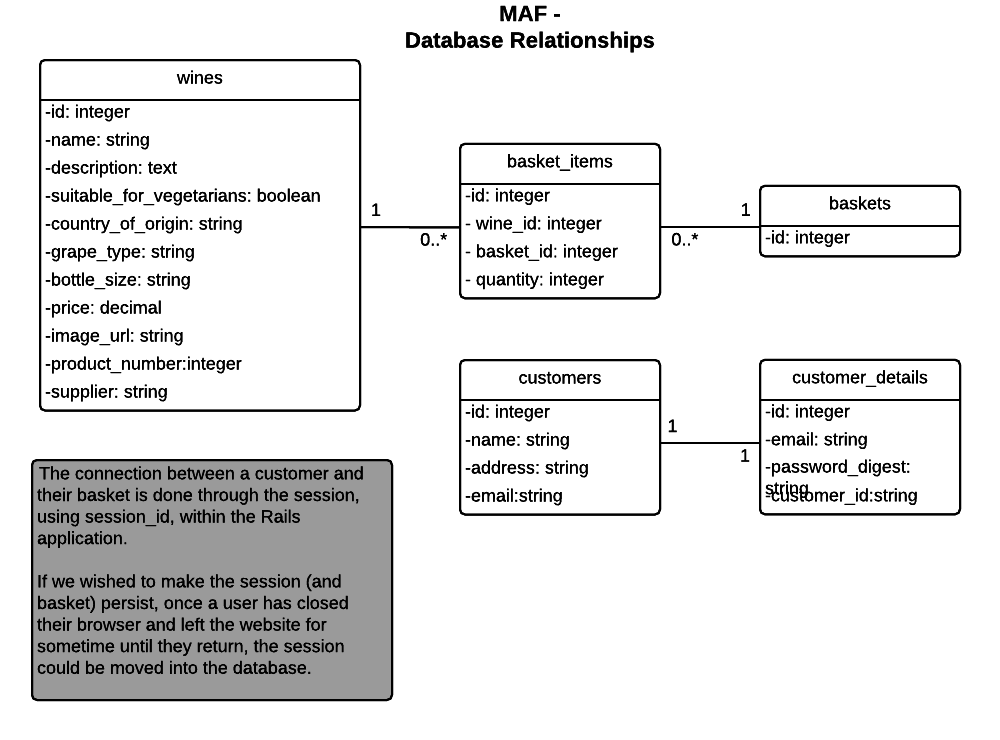
\includegraphics[width=1\textwidth]{assets/MAF_Database_relationships}
                \caption{The intended design of the database and relations between tables in the MAF application.}
                \label{fig: Intended MAF Database relationships.} 
\end{figure}

The representation of a BasketItem is for a many-to-many relationship, indicating that a Basket can have many Wines in it, and an Wine can be in many Baskets of different Customers. The connection between Customers and their Basket is done through the session parameter in Rails. I did consider having Session as an entity for storing in the database, and this would allow a user to retain their Basket and BasketItems for another time when they next login. However, I felt this was out of scope for the prototype and decided it was okay to have the basket be emptied and removed when a Session is ended. This leaves the session parameter containing the Basket id for a customer, and if they are logged in also their id and email, to make the join between the two.

I chose to keep the Supplier name as a field in the Wine entity, and the connections to these Suppliers is located in a configuration file. This could allow Suppliers to be updated through configuration once the site is hosted. However, I also know that there is the possibility of having a Table in the database for Web Suppliers which could contain their addresses, names and any additional needed information. Were I to re-implement this application, I may opt for that approach should more information about the Suppliers be required.

Based on what I expected to need, I made the target class design diagram that can be seen below. This shows the connections between the requests to MAF controllers and what the controllers connect to for their data and showing it.

\begin{figure}[H]
        \centering
                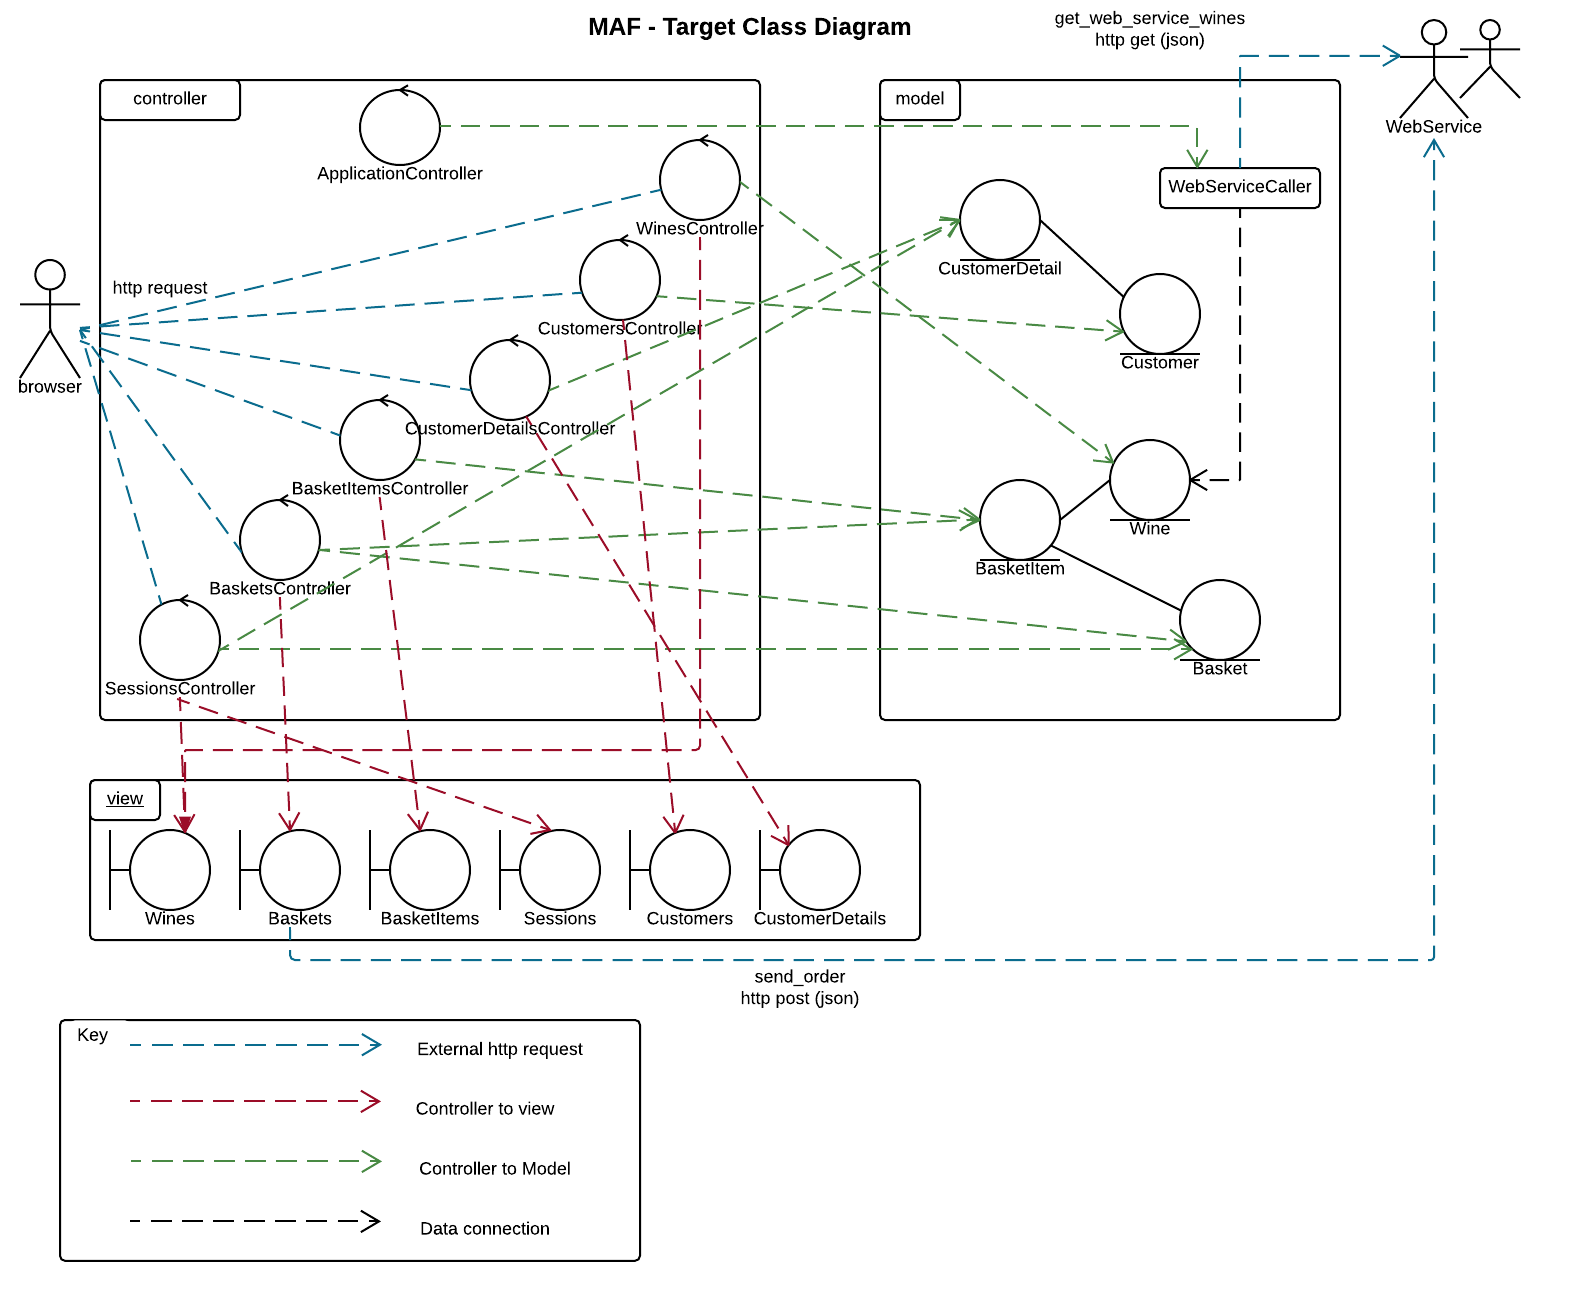
\includegraphics[width=0.8\textwidth]{assets/MAF_Target_Class_Design}
                \caption{The intended design of the classes and their connections in the MVC pattern.}
                \label{fig: Target Class Diagram.} 
\end{figure}

You can see that the SessionsController interacts with the Basket and CustomerDetail model, in order to keep the customer logged in with a persistent basket while they browse.

To get the Wines, calls are scheduled to be made every 60 seconds, using rufus-scheduler gem\cite{rufus} and are made asynchronously with SuckerPunch gem\cite{suckerpunch}, from my own class WebServiceCaller. This ensures that a user is not interrupted while they browse and the Wines are always kept up to date without making calls to the Web Suppliers too frequently. The WebServiceCaller gets the list of Wines from the Web Services listed in config, checks to see if the Wine is cheaper from a different supplier than the one known and makes this the new version of that Wine if it is. Otherwise it just confirms there are updates to the Wine given and updates it if there are. 

When we get the Wines from the Web Service, I chose only to get the image url, that matched with images already in MAF, rather than to link back to the Web Service. Through doing this, it leaves the application open to be able to be expanded upon later to get an actual copy of the images and store them in assets. I feel this is a better choice than linking back to the original images, as the bandwidth usage would increase on the Supplier web site through our image link back to them.

In order to fulfill the functional requirement of Search, I decided to use Solr with the Sunspot gem \cite{solrsunspot}. This allows for fulltext search and partial text search using NGrams, through any fields set as `searchable' on an entity. The allowing of partial search needs to be set up in the scheme configuration of Solr in order to work, but is very powerful once it is running. In order to use Solr, we must set up a local Solr server to use, and allow it to reindex for our records in order to find them.
\begin{lstlisting}
bundle exec rake sunspot:solr:start # or sunspot:solr:run
rake sunspot:reindex
\end{lstlisting}

Sending Orders to the Web Service is as simple as when a Customer clicks Checkout (while logged in), the order is sent to a method where a JSON body is built into a POST request for each Wine, and the order(s) is then sent to the respective suppliers of the Wines requested by the order. In a future version of the application, it would be preferable to have Orders kept in the database, to allow a Customer to see their previous orders.

%----------------------------------------------------------------------------------------
%	WEB SERVICE ARCHITECTURE
%----------------------------------------------------------------------------------------

\section{Web Service Architecture}

Since I was new to Rails, I chose to start developing my Web Service first, using Rails, to get comfortable with Ruby and the Rails framework. The Web Service only needed to know about two things, Wines and Orders, with RESTful routes to access what is needed for them, in this case a GET for wines.json, and POST for orders, to place an order and store it in the database.

\begin{figure}[H]
        \centering
                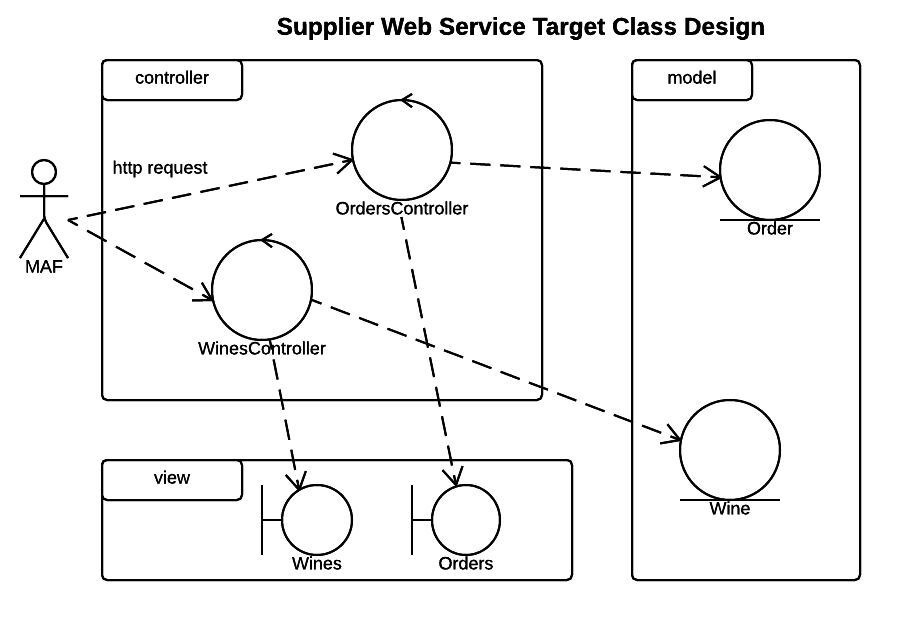
\includegraphics[width=1\textwidth]{assets/Supplier_Web_Service_Target_Class_Design}
                \caption{The intended design of the classes and their connections in the MVC pattern.}
                \label{fig: Target Class Diagram.} 
\end{figure}

Using RESTful endpoints, we don't need to define specific routes for certain things, and can just let Rails handle it, as long as we define that Orders and Wines are resources. When getting the Wine data, a GET request comes from MAF to the WinesController with a http header for when the service was last accessed by the MAF. The Web Service then gets all Wines in the database that were created or updated after the time MAF last asked for them and returns them in JSON format, along with its name, e.g.
\begin{lstlisting}
{"id":14,"name":"Abracadabwine","description":"Better than Magic! Tasty!","image_url":"wine6.jpg","price":"5.01","country_of_origin":"Poland","grape_type":"Green","suitable_for_vegetarians":true,"bottle_size":"350ml","url":"http://localhost:3001/wines/14.json","supplier":"Wine Supplier A"}
\end{lstlisting}

Doing this cuts down on the amount of database operations on the MAF side, and the bandwidth used by the Supplier. I originally had a method for deleting Wines no longer existing in any Web Service. This worked well for removing Wines that a supplier no longer displayed on their own website, until I implemented the check to only send wines that had been created or updated since I last called it. The delete function then started deleting all Wines in MAF except those updated.

I commented out the function, as it is no longer able to be used with the way I have implemented the communication between the MAF and Web Services, but left it in the code base for potential future reuse. However, if I were to do this again, I would have a flag on each Wine sent by the Web Service that says what status it is in (In Stock, Out of Stock, Discontinued) and use this flag to determine whether to keep or delete a Wine from the MAF database.

When it comes to receiving Orders, the Web Service receives a body of JSON that it parses into an Order entity and puts into the database, which is enough for this prototype. Each order contains the required customer information, the ID of the Wine in the Web Supplier (saved as 'Product Number' in MAF) and the quantity of the Wine to be ordered. I included a view for the Orders so I could see that the Orders were correctly sent by MAF.


%----------------------------------------------------------------------------------------
%	TEST STRATEGY
%----------------------------------------------------------------------------------------

\section{Test Strategy}
\subsection{System Testing}
My main focus for testing my system was the System Test Table. I wanted to be sure that my system met all of the functional requirements. I wrote my system test table and gradually went through them one by one to ensure my system passed them. Some of the tests I added but were slightly out of scope for this prototype, but I wished to include them as stretch goals.
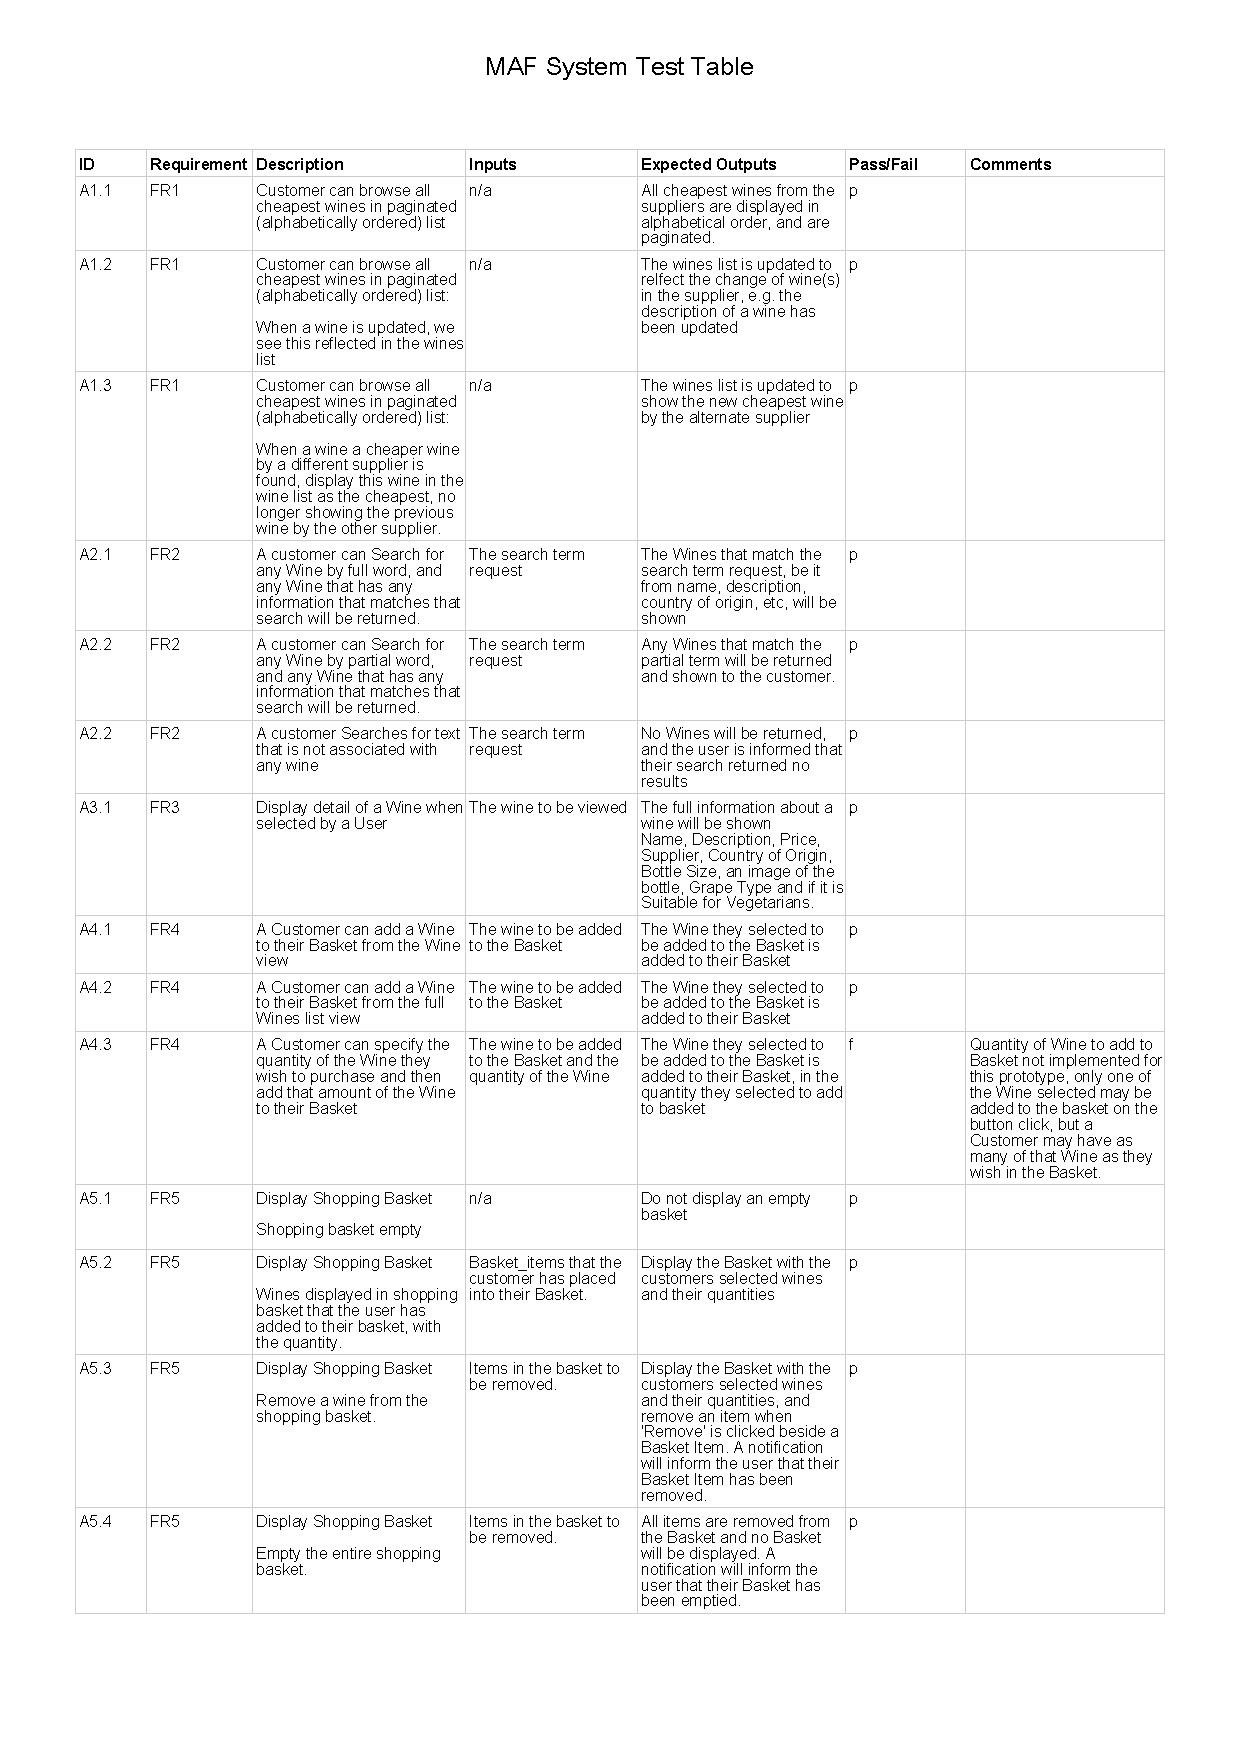
\includepdf[pages=-]{assets/MAF_System_Test_Table.pdf}
There are examples of the functional requirements laid about by the System Test Table shown below.

\begin{figure}[H]
        \centering
                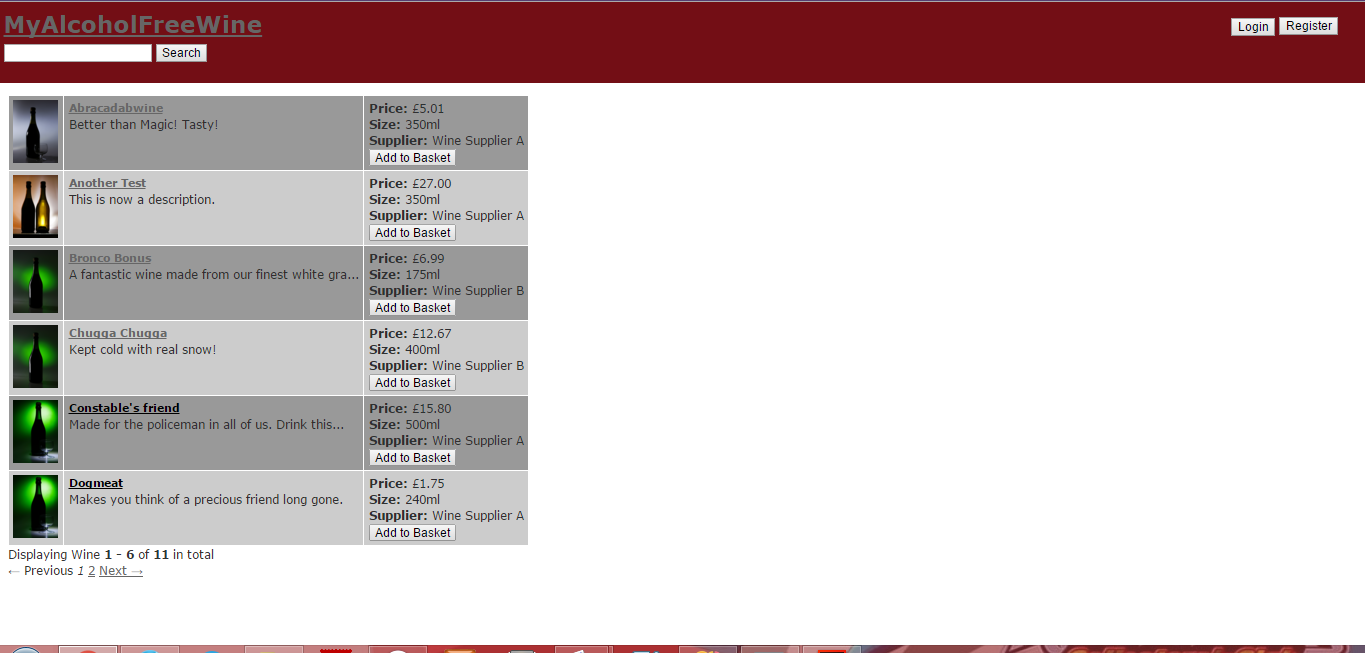
\includegraphics[width=1\textwidth]{assets/FR1_screen_1}
                \caption{FR1 - Displaying a list of cheapest Wines.}
                \label{fig: FR1_1.} 
\end{figure}

\begin{figure}[H]
    \centering
    \begin{subfigure}[b]{0.3\textwidth}
        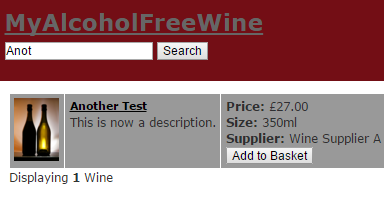
\includegraphics[width=\textwidth]{assets/FR2_screen_1}
        \caption{Search using partial text to find a Wine}
        \label{fig:FR2 partial}
    \end{subfigure}
    ~ %add desired spacing between images, e. g. ~, \quad, \qquad, \hfill etc. 
      %(or a blank line to force the subfigure onto a new line)
    \begin{subfigure}[b]{0.3\textwidth}
        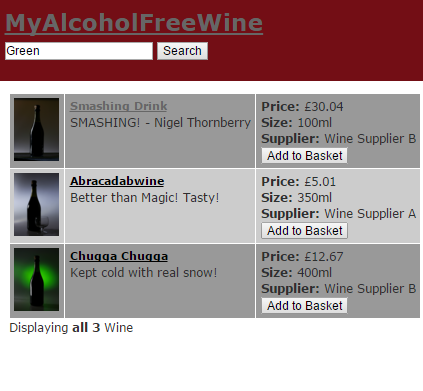
\includegraphics[width=\textwidth]{assets/FR2_screen_2}
        \caption{Searching Green for Grape Type}
        \label{fig:FR2 full search}
    \end{subfigure}
    ~ %add desired spacing between images, e. g. ~, \quad, \qquad, \hfill etc. 
    %(or a blank line to force the subfigure onto a new line)
    \begin{subfigure}[b]{0.3\textwidth}
        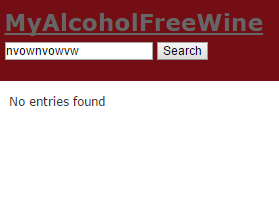
\includegraphics[width=\textwidth]{assets/FR2_screen_3}
        \caption{Searching something that won't give results}
        \label{fig:FR2 nonsense}
    \end{subfigure}
    \caption{FR2: Using the Search bar}\label{fig:FR2 Search}
\end{figure}

\begin{figure}[H]
        \centering
                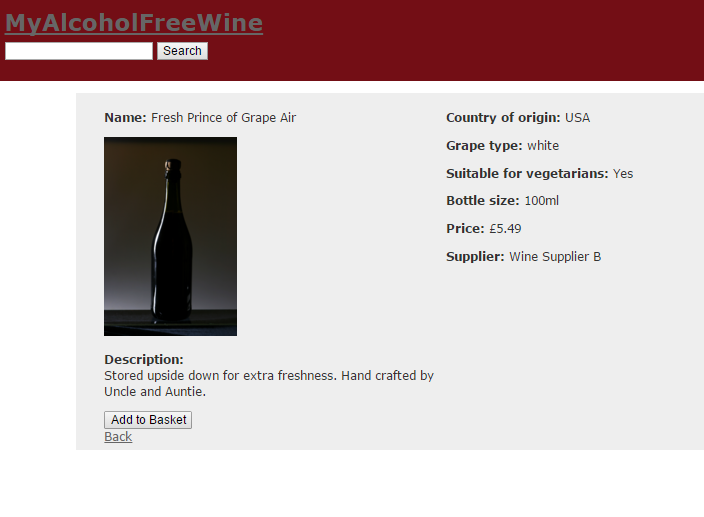
\includegraphics[width=1\textwidth]{assets/FR3_screen}
                \caption{FR3 - Displaying the full info for a Wine, FR4 allowing the Wine to be added to the Basket.}
                \label{fig: FR3_1.} 
\end{figure}

\begin{figure}[H]
    \centering
    \begin{subfigure}[b]{0.3\textwidth}
        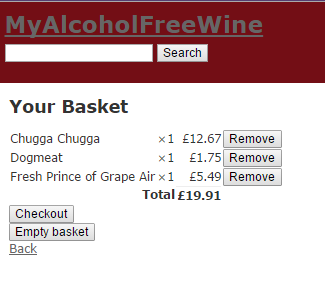
\includegraphics[width=\textwidth]{assets/FR5_screen_1}
        \caption{Viewing the Basket with items}
        \label{fig:FR5 view Basket}
    \end{subfigure}
    ~ %add desired spacing between images, e. g. ~, \quad, \qquad, \hfill etc. 
      %(or a blank line to force the subfigure onto a new line)
    \begin{subfigure}[b]{0.3\textwidth}
        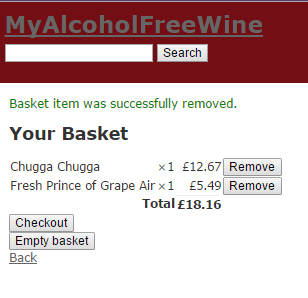
\includegraphics[width=\textwidth]{assets/FR5_screen_2}
        \caption{Remove item from Basket}
        \label{fig:FR5 Remove item from Basket}
    \end{subfigure}
    ~ %add desired spacing between images, e. g. ~, \quad, \qquad, \hfill etc. 
    %(or a blank line to force the subfigure onto a new line)
    \begin{subfigure}[b]{0.3\textwidth}
        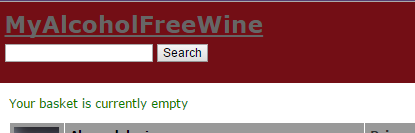
\includegraphics[width=\textwidth]{assets/FR5_screen_3}
        \caption{Emptying the Basket}
        \label{fig:FR5 empty basket}
    \end{subfigure}
    \caption{FR5: Interacting with the Basket}\label{fig:FR5 Basket}
\end{figure}

\begin{figure}[H]
        \centering
                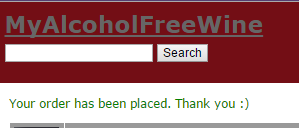
\includegraphics[width=1\textwidth]{assets/FR6_screen1}
                \caption{FR6 - Checking out.}
                \label{fig: FR6_1.} 
\end{figure}

\begin{figure}[H]
    \centering
    \begin{subfigure}[b]{0.3\textwidth}
        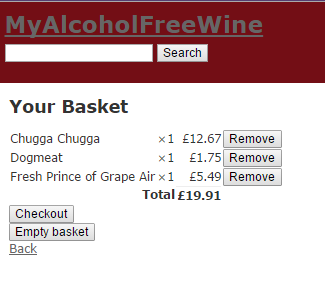
\includegraphics[width=\textwidth]{assets/FR5_screen_1}
        \caption{Viewing the Basket with items}
        \label{fig:FR5 view Basket}
    \end{subfigure}
    ~ %add desired spacing between images, e. g. ~, \quad, \qquad, \hfill etc. 
      %(or a blank line to force the subfigure onto a new line)
    \begin{subfigure}[b]{0.3\textwidth}
        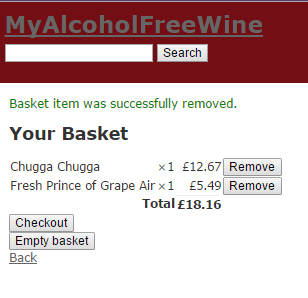
\includegraphics[width=\textwidth]{assets/FR5_screen_2}
        \caption{Remove item from Basket}
        \label{fig:FR5 Remove item from Basket}
    \end{subfigure}
    ~ %add desired spacing between images, e. g. ~, \quad, \qquad, \hfill etc. 
    %(or a blank line to force the subfigure onto a new line)
    \begin{subfigure}[b]{0.3\textwidth}
        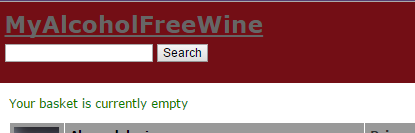
\includegraphics[width=\textwidth]{assets/FR5_screen_3}
        \caption{Emptying the Basket}
        \label{fig:FR5 empty basket}
    \end{subfigure}
    \caption{FR5: Interacting with the Basket}\label{fig:FR5 Basket}
\end{figure}



\subsection{Unit Test for models and controllers}
For testing the innards of my application, I used Rails unit testing for my models and controllers. Some of the generated tests by Rails were no longer required, as I didn't need actions for things such as New for Wines, as they are added into the database by the WebServiceCaller and not required to be added manually in MAF.

The majority of my Controller unit tests are ensuring that new objects are created when requesting, and importantly that the user is redirected to where they need to go. An example is when a User creates a basket item (adding an item to a Basket). I don't want a user to go to the Basket items list and see a bunch of items from all Baskets, and so they are instead redirected to their particular Basket\_path.

My unit tests for the models are mainly checking the validation, that no entities will be created that violate the conditions of their existence or creation. This ensures things a Customer always having an email address, and that it is unique to itself. 

\begin{figure}[H]
        \centering
                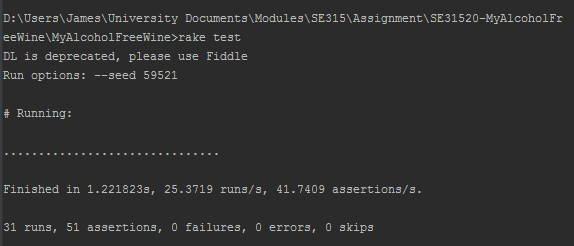
\includegraphics[width=1\textwidth]{assets/unit_test}
                \caption{Asking rake to run all test for my MAF project.}
                \label{fig: running tests.} 
\end{figure}

%----------------------------------------------------------------------------------------
%	SELF-EVALUATION
%----------------------------------------------------------------------------------------

\section{Self-Evaluation}
\subsection{Mark Breakdown}
\subsubsection{Screen cast}
Showed 2 Web Service Suppliers running, showed MAF running with all functionality discussed in this report. Expanded on this to show tests passing, Search in depth, etc Showed orders being received by the web suppliers
Mark: /10\%

\subsubsection{Design}
Design diagrams for both how I expected MVC to look and also for my database ideas, along with improvements. Explanation for my designs present and meeting the requirements, backed up through screen cast. Documentation quality is okay, could be more in-depth, and design could be improved, but I'm new to Rails and need more experience.
Mark: /20\%

\subsubsection{Implementation: MAF}
Application runs, and meets the requirements (except quantity indicator when adding to basket). Rails controllers make calls to models, and views receive the data from the controllers in order to display it. Code is commented, attributions to code where used and identifier names speak for themselves.
Mark: /25\%

\subsubsection{Implementation: Web Service}
Web Services run, code has comments and names are good. RESTful resources, wines and orders, can call them and the routing sends the request to the controller through the type of request.
Mark: /15\%

\subsubsection{Testing}
Unit tests for each controller, more than just the ones generated by rails, and tests for the models, validations and own methods too. System test table matches assumed customer expectations. Results are discussed and based on these what could be taken forward if this prototype were to be fully implemented
Mark: /15\%

\subsubsection{Evaluation}
Full evaluation of report, MAF and web service, with summary of evaluation below the mark breakdown, with what was learned, difficult and easy.
Mark: /5\%

\subsubsection{Flair}
Implementation of Search using Solr with Sunspot to search partial words from all sections, editing the schema to change the gram of the search. Calling the WebService asynchronously with SuckerPunch, scheduling it to update with rufus-scheduler for hands off updating without interrupting the customer as they browse the website. Only retrieving the latest updates to wines to cut costs on database operations.
Mark: /10\%

\subsubsection{Total}
Mark: /100\%

\subsection{Summary}
I think I met all of the functional requirements as requested, and the resources as RESTful and data is represented in the Rails way. I know there are areas for improvement (security, clean up, persistent sessions and baskets, better tests, cucumber tests, etc), but as far as the time allowed, my understanding and learning of Rails and this assignment tasking me to just create a prototype, I am happy with the resulting program, and happy I could learn more about Rails and Ruby, how to implement an MVC pattern, talking between web services and even implement external features, like learning configurations of Solr for my search.

I found the most difficult part to be implementing routing, and getting my links in the views to execute the correct controller actions as I wanted (for the more complex tasks, such as removing the last item from a basket, logging in and sending the webservice order). Before this assignment I had little working knowledge of rails outside of the workshops and a small amount of experience with routing, and doing this assignment helped me get my head around routing and how it works, and has helped me feel comfortable going forward in the future to building more Rails apps when I want to make a web application. 



%----------------------------------------------------------------------------------------
\clearpage

%----------------------------------------------------------------------------------------
%	REFERENCES
%----------------------------------------------------------------------------------------

\begin{thebibliography}{5}

\bibitem{assignment} Chris Loftus, ``MyAlcoholFreeWine.com'',SE31520/CHM5820 Assignment 2015-16, October 27 2015

\bibitem{stockvault} Stockvault.net, 'Stockvault.net - Free wine Stock Photos', 2015. [Online]. Available: http://www.stockvault.net/search/?query=wine. [Accessed: 06- Dec- 2015].

\bibitem{railsbook} D. Thomas, D. Hansson and L. Breedt, Agile web development with rails. Raleigh, N.C.: Pragmatic Bookshelf, 2005.

\bibitem{rufus} GitHub, 'jmettraux/rufus-scheduler', 2015. [Online]. Available: https://github.com/jmettraux/rufus-scheduler. [Accessed: 06- Dec- 2015].

\bibitem{suckerpunch} GitHub, 'brandonhilkert/sucker\_punch', 2015. [Online]. Available: https://github.com/brandonhilkert/sucker\_punch. [Accessed: 06- Dec- 2015].

\bibitem{solrsunspot}  Sunspot.github.io, 'Sunspot: Solr-powered search for Ruby objects', 2015. [Online]. Available: http://sunspot.github.io/. [Accessed: 06- Dec- 2015].

\end{thebibliography}


\end{document}


